% Created 2022-11-09 mié 11:36
% Intended LaTeX compiler: pdflatex
\documentclass[12pt]{article}
\usepackage[utf8]{inputenc}
\usepackage[T1]{fontenc}
\usepackage{graphicx}
\usepackage{grffile}
\usepackage{longtable}
\usepackage{wrapfig}
\usepackage{rotating}
\usepackage[normalem]{ulem}
\usepackage{amsmath}
\usepackage{textcomp}
\usepackage{amssymb}
\usepackage{capt-of}
\usepackage{hyperref}
\usepackage[spanish]{babel}
\usepackage{graphicx,geometry}
\geometry{ a4paper, left=1in, right=1in, top=1in, bottom=1in }
\renewcommand\familydefault{\sfdefault}
\usepackage{sectsty}
\sectionfont{\normalfont\Large }
\subsectionfont{\normalfont}
\usepackage{tabularx}
\usepackage{listings}
\lstdefinestyle{mystyle}{
numbers=left,
showspaces=false,
frame=leftline,
showspaces=false,
showstringspaces=false,
showtabs=false,
numberstyle=\tiny,
}
\lstset{
style=mystyle,
literate={á}{{\'a}}1
{é}{{\'e}}1
{í}{{\'{\i}}}1
{ó}{{\'o}}1
{ú}{{\'u}}1
{Á}{{\'A}}1
{É}{{\'E}}1
{Í}{{\'I}}1
{Ó}{{\'O}}1
{Ú}{{\'U}}1
{ü}{{\"u}}1
{Ü}{{\"U}}1
{ñ}{{\~n}}1
{Ñ}{{\~N}}1
{¿}{{?``}}1
{¡}{{!``}}1
}
\makeatletter
\usepackage{fancyhdr}
\pagestyle{fancy}
\usepackage{mdframed}
\BeforeBeginEnvironment{minted}{\begin{mdframed}}
\AfterEndEnvironment{minted}{\end{mdframed}}
\author{Luis Eduardo Galindo Amaya (1274895)}
\date{04-11-2022}
\title{Interrupciones}
\hypersetup{
 pdfauthor={Luis Eduardo Galindo Amaya (1274895)},
 pdftitle={Interrupciones},
 pdfkeywords={},
 pdfsubject={},
 pdfcreator={Emacs 26.3 (Org mode 9.1.9)}, 
 pdflang={Spanish}}
\begin{document}



\newcommand{\docente}{Arturo Arreola Alvarez}
\newcommand{\asignatura}{Organización de Computadoras (331)}
\newcommand{\semestre}{2022-2}

\newcommand{\miportada}[1]{
	\begin{titlepage}
		\vspace*{0.75in}
		\begin{flushleft}
			\sffamily
			\large #1       \\
			\Huge 
            \@title         \\
			\hrulefill
			\vspace{0.25in} \\
			\Large \@author \\
			\vspace*{\fill}
            
\includegraphics[width=\textwidth]{../includes/filler.png} \\
			\vspace*{\fill}
			\large
			\begin{tabular}{|l|l|}
              \hline
			  Asignatura & \asignatura \\
			  Docente    & \docente    \\
			  Fecha      & \@date      \\
              \hline
			\end{tabular}
		\end{flushleft}
	\end{titlepage}
}

\miportada{ Práctica 10 }

\fancyhf{}
\lhead{ \asignatura }
\rhead{ \semestre }
\rfoot{Página \thepage}

\setlength\parindent{0pt}   % eliminar el intentado
\setlength{\parskip}{1.2em}
\maketitle

\section*{Objetivo}
\label{sec:orgbd4fac0}
Seleccionar las instrucciones de llamadas al sistema adecuadas, para 
desarrollar aplicaciones de sistemas basados en microprocesador, 
mediante el análisis de su funcionalidad, de forma responsable y eficiente.

\section*{Desarollo}
\label{sec:org7ccdc2f}
\subsection*{Actvidad 1}
\label{sec:orge9d07a3}
Completar la tabla sobre los parámetros necesarios en las llamadas al
sistema operativo para el manejo de archivos en Linux por medio de la 
interrupción 80h.

\begin{center}
\begin{tabular}{|l|l|l|}
\hline
Servicio & Param. del servicio & Explicación\\
\hline
 & EAX = 3 & Numero del servicio\footnotemark\\
Leer & EBX = 0 & Unidad de entrada\footnotemark\\
 & ECX = ptr & puntero a un área de memoria\\
 & EDX = length & Número de caracteres a leer\\
\hline
 & EAX = 4 & Numero del servicio\\
Escribir & EBX = 1 & unidad de salida\footnotemark\\
 & ECX = ptr & Puntero a un área de memoria\\
 & EDX = lenght & Número máximo de caracteres\\
\hline
 & EAX = 5 & Numero del servicio\\
Abrir & EBX = path & Dir. de una cadena de caracteres\\
 & ECX = mode & Modo de acceso\footnotemark\\
 & EDX = permisos & Permisos al archivo\\
\hline
\end{tabular}
\end{center}\footnotetext[1]{\label{orgde44e8b}al terminar el servicio el valor se reemmplaza con el numero de caracteres capturados}\footnotetext[2]{\label{org98a730b}0: Entrada estándar o teclado.}\footnotetext[3]{\label{orge08a8aa}1: salida estándar o terminal.}\footnotetext[4]{\label{org1192bcc}Más informacion: \url{https://es.wikipedia.org/wiki/Int\_80h}}

\subsection*{Actividad 2}
\label{sec:orgf153df1}
Codifique las funciones gets y puts las cuales capturan e imprimen una 
cadena de caracteres en pantalla, respectivamente. Solo haga uso de la 
interrupción 80h. No haga uso de la librería proporcionada.

\begin{description}
\item[{La subrutina gets}] solo debe poder capturar la cantidad máxima de caracteres que caben en el buffer en el que se guardará la cadena.

\item[{La subrutina puts}] debe ser capaz de detectar la longitud de la cadena a imprimir y pasar este valor a la interrupción 80h para establecer la cantidad de  caracteres a imprmir.
\end{description}

\subsection*{Actividad 3}
\label{sec:org42bb9d7}
Cree un archivo dentro de la misma carpeta, llamado P10.txt. Dentro de
este archivo, coloque su nombre y su matrícula. Desarrolle una subrutina
que le permita leer el contenido del archivo e imprimirlo en pantalla
utilizando la interrupción 80h. Mencione que datos se deben colocar en
cada registro para lograr esto. 

\section*{Captura}
\label{sec:orgd612cb4}
\begin{center}
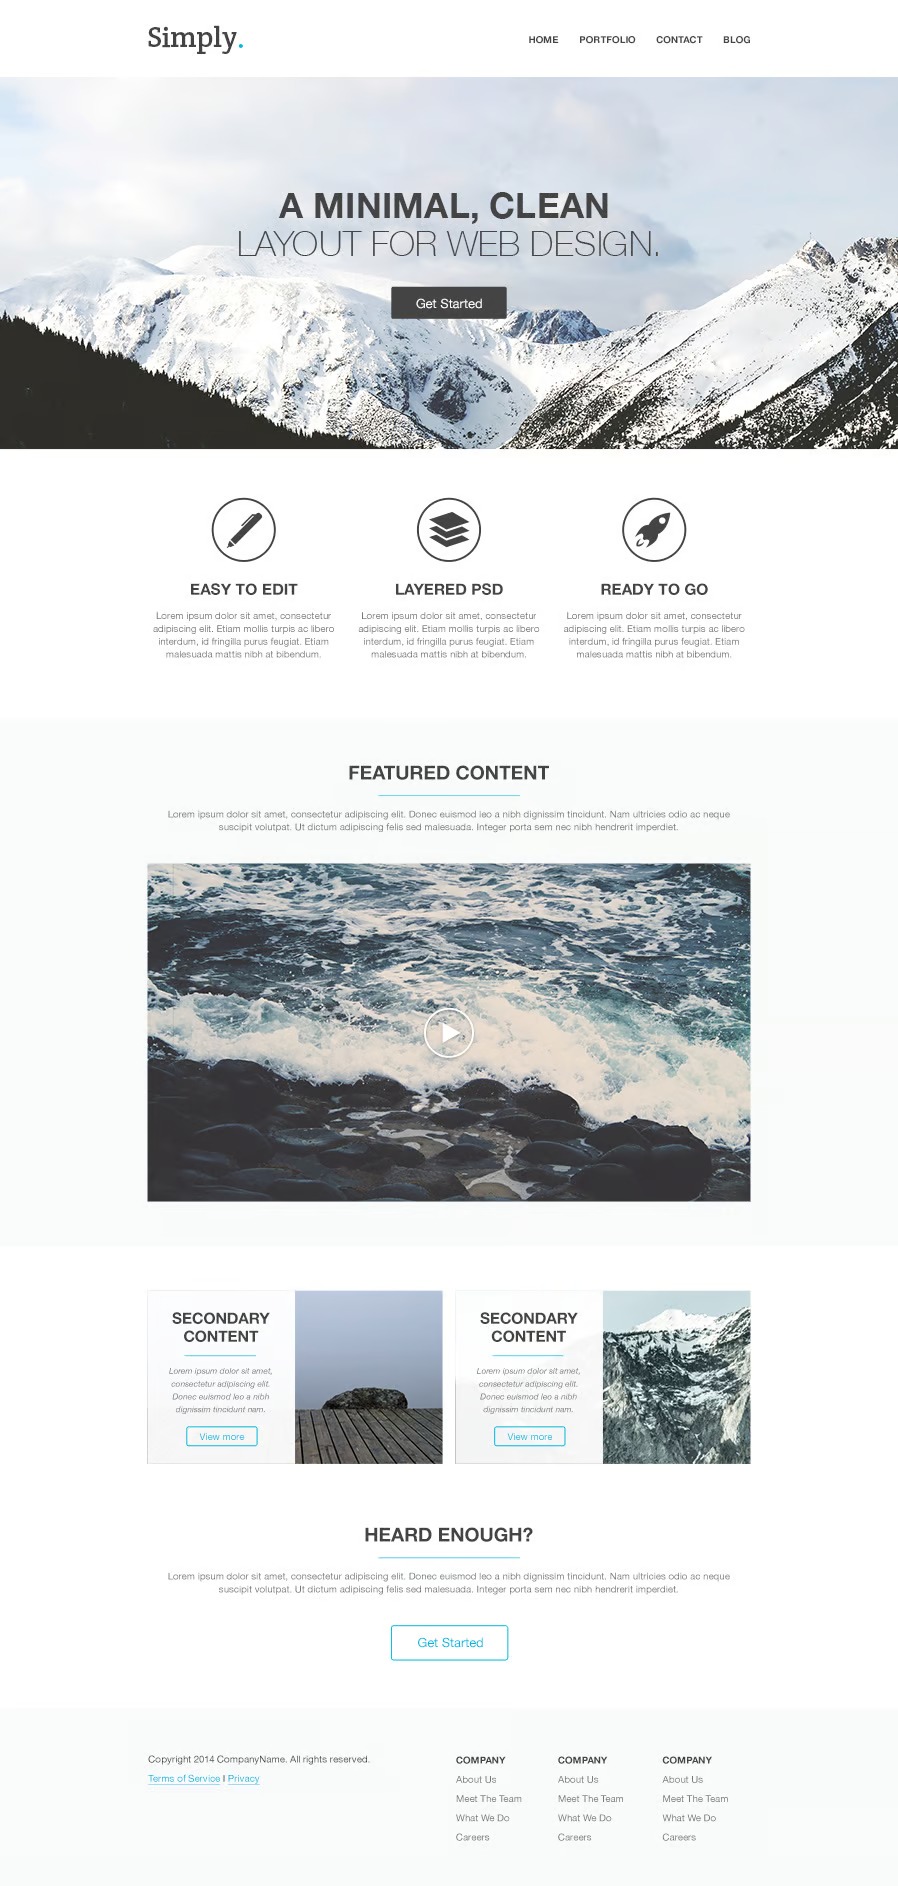
\includegraphics[width=.9\linewidth]{img/a.png}
\end{center}

\section*{Conclusiones}
\label{sec:org0691a3a}
Cuando trabajamos con interrupciones lo principal cosa que debemos tomar en cuenta
es que cada sistema operativo es diferente, por lo que nuestro código va a tener
que modificarse de acuerdo a cada sistema operativo lo cual añade una capa mas
a las complicaciones que requiere el ensamblador para funcionar.

\section*{Dificultades}
\label{sec:org7bad91b}
Con la interrupción de captura tuve que añadir una funcion para vaciar el 
buffer, ya que pasaba los valores a la siguiente captura.

\section*{Código}
\label{sec:org49f55d7}
\\ \lstinputlisting{./src/P10.asm}

\section*{Fuentes}
\label{sec:orgb2dad22}
\begin{description}
\item[{Lista de interrupciones}] \url{https://es.wikipedia.org/wiki/Int\_80h}
\item[{Descripciones de las interrupciones}] \url{http://www.int80h.org/}
\item[{Leer un archivo e imprimir el contenido}] \url{https://stackoverflow.com/q/26963871}
\item[{Mover un valor desde .data a un registro}] \url{https://stackoverflow.com/a/64005239}
\item[{Generalidades de NASM}] \url{https://shorturl.at/lsuHS}
\item[{Direccion en un arreglo}] \url{https://reverseengineering.stackexchange.com/a/18711}
\end{description}
\end{document}
